\chapter{Estado de Arte}

En esta secci\'on vamos a pasar revista de una serie de tecnolog\'ias
investigadas o testeadas durante la tesis. La primera, IBM-Watson es
quiz\'as la m\'as conocida para el p\'ublico en general. 


//write stuff\newline


\section{IBM-Watson}

Watson es un sistema dise\~nado por IBM con el objetivo de competir en
tiempo real en el programa de televisi\'on estadounidense Jeopardy,
logrando resultados del nivel de los campeones humanos de este
programa.

El proyecto demor\'o 3 a\~nos de investigaci\'on, en los cuales se
logr\'o obtener la performance esperada (nivel humano experto) en
cuanto a precisi\'on, confiabilidad y velocidad, logrando derrotar a
dos de los hombre con mayores r\'ecords hist\'oricos del show en un
programa en vivo [M\'AS DATOS -LINKS]

El objetivo del \ proyecto puede considerarse una extensi\'on de lo que
fue Deep Blue, el sistema que logr\'o el nivel de los expertos humanos
en el ajedrez, porque busc\'o superar un reto que significativo y
visible del campo de la Inteligencia Artificial tanto para la comunidad
cient\'ifica como para la sociedad en general:
{\textquotedblleft}?`puede un sistema computacional ser dise\~nado para
competir con los mejores hombre en alguna tarea que requiera altos
niveles de inteligencia humana y, si es el caso, que clase de
tecnolog\'ia, algoritmos e ingenieria se
requiere?{\textquotedblright}\footnote{\ Traducci\'on propia de
Building Watson: An Overview of the DeepQA Project, p2}

Watson es la implementaci\'on espec\'ifica para participar en este
programa de una arquitectura m\'as gen\'erica de question answering,
DeepQA, que da el nombre al proyecto de la corporaci\'on. Esta
arquitectura ejemplifica perfectamente la complejidad del problema de
QA de dominio abierto e incorpora tecnolog\'ias de punta de distintos
dominios de ciencias de la computaci\'on, y de IA en particular:
information retrieval, natural language processing, knowledge
representation and reasoning, machine learning e interfaces humano -
computadora.

\subsection{El problema}

Watson debe realizar tareas como parsing, question classification,
question descomposition, automatic source adquisition and evaluation,
entity and relation detection, logical form generation, knowledge
representation and reasoning manteniendo ciertos atributos de calidad
bastante exigentes derivados de la naturaleza del show. Estas
restricciones son:

\begin{itemize}
\item Confiabilidad de la respuesta: \newline
Jeopardy tiene tres participantes con un pulsador y el que desee
responder debe pulsar antes que los dem\'as. Adem\'as, existe una
penalizaci\'on por respuestas incorrectas, por lo que es esencial que
el sistema pueda determinar la confiabilidad de la respuesta obtenida a
fin de optar por responder o no responder.
\item Tiempos de respuesta: \newline
La confiabilidad de la respuesta, o al menos una estimaci\'on, debe
calcularse antes de que pase el tiempo para decidir responder (6
segundos) y tambi\'en de que otro participante oprima su pulsador
(menos de 3 segundos).
\item Precisi\'on:\newline
El tipo de respuestas que se dan en el show suelen ser respuestas
exactas (por ejemplo: solamente un nombre, un n\'umero o una fecha,
etc). 
\end{itemize}

\bigskip

El sistema cuenta con varios componentes heur\'isticos que estiman
ciertos features y grados de confiabilidad para diferentes respuestas,
los cuales son evaluados por un sistema general que sintetiza un grado
de confiabilidad para una respuesta final y determina as\'i si
responder o no responder. 

El programa consta de un tablero con 30 pistas (o preguntas) organizadas
en seis columnas, cada una de las cuales es una categor\'ia. Las
categor\'ias van desde temas acotados como
{\textquotedblleft}historia{\textquotedblright} o
{\textquotedblleft}ciencias{\textquotedblright} hasta temas m\'as
amplios como {\textquotedblleft}cualquier cosa{\textquotedblright} o
{\textquotedblleft}potpourri{\textquotedblright}. Watson intenta
respuestas sobre varias hip\'otesis de dominio y verifica en cual de
ellos se logran respuestas de mayor confiabilidad. 

Por otra parte, el grueso de las preguntas de Jeopardy son del tipo
\textit{factoid}, esto es, preguntas cuya respuesta esta basada en
informaci\'on f\'actica acerca de una o m\'as entidades individuales.


\bigskip

Por ejemplo:

Categor\'ia: Ciencia General

Pista: Cuando es impactado por electrones, un f\'osforo emite energ\'ia
electromagn\'etica de esta forma

Respuesta: Luz (o fotones)


\bigskip

A su vez, existen ciertos tipos de pistas que requieren un enfoque
particular, por ejemplo, pistos que constan de dos subpistas muy
d\'ebilmente relacionadas, o problemas matem\'aticos formulados en
lenguaje humano, o problemas de fon\'etica, etc, que no pueden ser
simplemente dejados de lado porque, si bien tiene poca probabilidad de
aparici\'on, cuando aparecen lo hacen en bloque y pueden arruinar el
juego de Watson. Se acord\'o con la productora del programa, sin
embargo, dejar de lado preguntas audiovisuales (aquellas que presentan
una imagen o un audio y requieren interpretarlo) y preguntas que
requieren instrucciones verbales del presentador.


\bigskip

Para determinar el dominio de conocimiento, los investigadores
analizaron 20000 preguntas, extrayendo su LAT (lexical answer type, o
tipo l\'exico de respuesta). El LAT se define como una palabra en la
pista que indica el tipo de la respuesta esperado. Por ejemplo, para la
pista {\textquotedblleft}Investanda en 1500{\textquoteright}s para
agilizar el juego, este movimiento involucra dos
piezas{\textquotedblright} el LAT es
{\textquotedblleft}movimiento{\textquotedblright}. Menos del 12\% de
las pistas no indicaba expl\'icitamente ning\'un LAT, usando palabras
como {\textquotedblleft}esto{\textquotedblright} o
{\textquotedblleft}eso{\textquotedblright}. En estos casos, el sistema
debe inferir el tipo de respuesta del contexto. Del an\'alisis de estas
20000 pistas se reconocieron 2500 tipos l\'exicos distintos, de los
cuales los 200 m\'as frecuentes no llegaban a cubrir el 50\% del total
de pistas. Esto implica que un approach estructurado (orientado por el
tipo de respuesta), si bien resulta \'util para algunos tipos, no es
suficiente para abordar el problema completo.

\subsection{M\'etricas}

Las m\'etricas de resultados, adem\'as del tiempo de respuesta, son la
\textit{precisi\'on} (preguntas contestadas correctamente / preguntas
contestadas) y el \textit{porcentaje de respuestas dadas }(preguntas
contestadas / total de preguntas). Mediante la configuraci\'on de un
threshold de \textit{confiabilidad} pueden obtenerse distintas
estrategias de juego: un umbral bajo repercutir\'a en un juego m\'as
agresivo, incrementando la proporci\'on de respuestas contestadas,,
pero disminuyendo su precisi\'on, mientras que un umbral alto
determinar\'a un juego conservador, con menos respuestas dadas pero
mayor precisi\'on en las mismas. Es un cl\'asico escenario de trade-off
entre dos atributos de calidad. Un buen sistema de estimaci\'on de
confiabilidad implica una mejora general del sistema, a\'un cuando el
m\'odulo de generaci\'on de respuestas permanezca id\'entico.


\bigskip

En el show, el porcentaje de respuestas dadas depende de la velocidad
con la que se llega a presionar el pulsador, lo cual s\'olo interesa
para el dominio de QA como una restricci\'on temporal. 


\bigskip

Mediante an\'alisis num\'erico, los investigadores determinaron que los
campeones de Jeopardy lograban tomar entre el 40\% y el 50\% de las
preguntas y, sobre ellas, lograban una precisi\'on de entre el 85\% y
el 95\%, lo que determinaba una barrera de performance bastante
exigente en lo que respecta a QA.


\bigskip

\subsection{Baseline}

El equipo de IBM intent\'o utilizar dos sistemas consolidados en QA y
adaptarlos al problema \ de Jeopardy. \ El primero fue PIQUANT
(Practical Intelligent Question Answering Technology), un sistema
desarrollado por IBM en conjunto con el programa del gobierno
estadounidense AQUAINT y varias universidades, que estaba entre los
mejores seg\'un la TREC (Text Retrieval Conference), una autoridad en
el \'area. PIQUANT consta de un pipeline t\'ipico (v\'ease QANUS) con
tecnolog\'ia de punta, logrando un rango del 33\% de respuestas
correctas en las evaluaciones TREC-QA. Los requerimientos de la
evaluaci\'on de TREC son muy distintos de los de Jeopardy: TREC ofrece
un corpus de conocimiento relativamente peque\~no (1M de documentos) de
donde las respuestas deben ser extra\'idas y justificadas, el tipo de
preguntas de TREC son menos complejas a nivel ling\"u\'istico que las
de Jeopardy y la estimaci\'on de confiabilidad no resulta una m\'etrica
importante (dado que no hay penalizaci\'on por respuestas incorrectas).
Adem\'as, los sistemas tienen permitido acceder a la web y las
restricciones temporales son, por mucho, m\'as amplias (por ejemplo:
una semana para responder 500 preguntas). En Jeopardy, adem\'as de las
restricciones ya mencionadas, un requerimiento fue que el sistema
trabaje sobre datos locales y no acceda a la web en tiempo real. El
intento de adaptar PIQUANT al problema de Jeopardy dio p\'esimos en
comparaci\'on con los necesarios: 47\% de precisi\'on sobre el 5\% de
respuestas con mayor confiabilidad y 13\% de precisi\'on en general. 

Por otro lado, el equipo intent\'o adaptar el sistema OpenEphyra
(v\'ease OpenEphyra), un framework open-source de QA desarrollado en
CMU (Carnegie Mellon University) basado en Ephyra (no libre),
dise\~nado tambi\'en para la evaluaci\'on TREC. OpenEphyra logra un
45\% de respuestas correctas sobre el set de datos de evaluaci\'on TREC
2002, usando busqueda web. La adaptaci\'on result\'o a\'un peor que la
de PIQUANT (con menos del 15\% de respuestas correctas y una mala
estimaci\'on de la confiabilidad). 

Se probaron dos adaptaciones de estos sistemas. una basada en
b\'usquedas de texto puro y otra basada en reconocimiento de entidades.
En la primera, la base de conocimiento se model\'o de manera no
estructurada y las preguntas se interpretaron como t\'erminos de una
query, mientras que en la segunda se model\'o una base de conocimientos
estructurada y las preguntas se analizaron sem\'anticamente para
reconocer entidades y relaciones, para luego buscarlos en la base.
Comparando ambos enfoques en base al porcentaje de respuestas dadas, el
primero dio mejores resultados para el 100\% de las respuestas,
mientras que la confiabilidad general era baja; por otro lado, el
segundo enfoque logr\'o altos valores de confiabilidad, pero s\'olo en
los casos en que efectivamente logra identificar entidades. De aqu\'i
se infiere que cada enfoque tiene sus ventajas, en el dominio de
problemas apropiado.

\subsection{La arquitectura DeepQA}
\label{subsec:deep-qa}
Los intentos de adaptaci\'on iniciales, como vimos, no dieron
resultados, as\'i como tampoco sirvieron las adaptaciones de algoritmos
de la literatura cient\'ifica, los cuales son realmente dif\'iciles de
sacar de su contexto original y de las evaluaciones sobre las cuales
fueron testeados. Este problema, veremos -por ejemplo, con QANUS y
Reverb- , se repiti\'o en nuestro proyecto. Como conclusi\'on de estos
intentos frustrados, el equipo de IBM entendi\'o que una arquitectura
de QA no deb\'ia basarse en sus componentes concretos sino en la
facilidad para incorporar nuevos componentes y para adaptarse a nuevos
contextos. As\'i surgi\'o DeepQA, la arquitectura de base, de la cual
Watson es una instancia concreta para un contexto particular (con
requerimientos de alta precisi\'on, buena estimaci\'on de
confiabilidad, lenguaje complejo, amplitud de dominio y restricciones
de velocidad). DeepQA es una arquitectura de computo paralelo,
probabilistico, basado en recopilaci\'on de evidencia y scoring. Para
Jeopardy se utilizaron m\'as de 100 t\'ecnicas diferentes para analizar
lenguaje natural, identificar y adjudicar valor a fuentes de
informaci\'on, encontrar y generar hip\'otesis, encontrar y rankear
evidencias y mergear y rankear hip\'otesis en funci\'on de esta
evidencia. La arquitectura sirvi\'o para ganar Jeopardy, pero tambi\'en
se adapt\'o a otros contextos como la evaluaci\'on TREC, dando
resultados mucho mejores que sus predecesores. Los principios de
dise\~no subyacentes de la arquitectura son:

\begin{itemize}
\item Paralelismo masivo\newline
Para evaluar distintas hip\'otesis en distintos dominios con poco
acoplamiento.
\item Pervasive confidence estimation:\newline
Ning\'un componente genera la respuesta final, sino que da una serie de
features y grados de confiabilidad y evidencia para distintas
hip\'otesis, que luego son sintetizados.
\item Integrate shallow and deep knowledge:
\end{itemize}

\bigskip

A continuaci\'on, enumeraremos la lista de pasos que sigue el sistema
para obtener la respuesta a una pregunta:

\subsubsection{Adquisici\'on de contenidos}

El primer paso de DeepQA es la adquisici\'on de contenidos. Este paso es
el \'unico que no se realiza en tiempo de ejecuci\'on y consiste en
crear la base de conocimiento en la cual el proceso final buscar\'a la
respuesta a la pregunta, combinando subprocesos manuales y
autom\'aticos. 

En principio se caracteriza el tipo de preguntas a responder y el
dominio de aplicaci\'on. El an\'alisis de tipos de preguntas es una
tarea manual, mientras que la determinaci\'on del dominio puede
encararse computacionalmente, por ejemplo, con la detecci\'on de LATs
que se\~nalamos antes. Dado el amplio dominio de conocimientos que
requiere Jeopardy, Watson cuenta con una gran cantidad de
enciclopedias, diccionarios, tesauros, art\'iculos acad\'emicos y de
literatura, etc. A partir de este corpus inicial, el sistema busca en
la web documentos relevantes y los relaciona con los documentos ya
presentes en el corpus. 

Adem\'as de este corpus de documentos no estructurados, DeepQA maneja
contenidos semi-estructurados \ y estructurados, incorporando bases de
datos, taxonom\'ias y ontolog\'ias como dbPedia, Wordnet y las
ontolog\'ias de Yago. 

\subsubsection{An\'alisis de la pregunta}

El primer paso en run-time es el an\'alisis de la pregunta. En este paso
el sistema intenta entender qu\'e es lo que la pregunta est\'a
preguntado y realizar los primeros an\'alisis que determinan c\'omo
encarar\'a el procesamiento el resto del sistema. Watson utiliza
shallow parses, deep parses, formas l\'ogicas, pos-tags,
correferencias, detecci\'on de entidades nombradas y de relaciones,
question classification, adem\'as de ciertos an\'alisis concretos del
domiento del problema.

En este proceso se clasifica el tipo de la pregunta (los tipos est\'an
determinados por el show: puzzles, matem\'aticos, etc). Tambi\'en se
busca el tipo de respuesta esperada, d\'onde los tipos manejados son
por Watson son los LATs extra\'idos de las preguntas de ejemplo. El LAT
determina el {\textquotedblleft}tipo{\textquotedblright} de la
respuesta, que clase de entidad \textit{es} la respuesta (una fecha, un
hombre, una relaci\'on, etc). El equipo de IBM intent\'o adaptar
distintos algoritmos de clasificaci\'on preexistentes, pero despu\'es
de intentar entrenarlos para el dominio de tipos de Jeopardy, llegaron
a la conclusi\'on de que su eficacia era dependiente del su sistema de
tipos default, y que la mejor forma de adaptaci\'on era mappear su
output a los tipos utilizados por Watson (un enfoque similar fue
utilizado en esta tesis con respecto al clasificador de Stanford). Otra
anotaci\'on importante es el
{\textquotedblleft}foco{\textquotedblright} de la pregunta, la parte de
la pregunta tal que si se la reemplaza por la respuesta, la pregunta se
convierte en una afirmaci\'on cerrada.

Por ejemplo, para {\textquotedblleft}El hombre que escribi\'o Romeo y
Julieta{\textquotedblright}, el foco es {\textquotedblleft}El hombre
que{\textquotedblright}. Este fragmento suele contener informaci\'on
importante sobre la respuesta y al reemplazarlo por una respuesta
candidata se obtiene una afirmaci\'on f\'actica que puede servir para
evaluar distintos candidatos y recolectar evidencia. Por ejemplo,
reemplazando por distintos autores y verificando que la oraci\'on
resultante est\'e presente en el corpus.

Por otro lado, muchas preguntas involucran relaciones entre entidades y,
m\'as puntualmente, tienen una forma sujeto-verbo-objeto. Por ejemplo,
tomando la pista anterior, podemos extraer la relaci\'on
\textit{escribir(x, Romeo y Julieta)}. La amplitud del dominio de
Jeopardy hace que la cantidad de entidad y de relaciones entre
entidades sea enorme, pero esto empeora a\'un m\'as al considerar las
distintas formas de expresar la misma relaci\'on. Por eso, Watson
s\'olo logra encontrar directamente una respuesta mediante
reconocimiento de entidades y relaciones sobre el 2\% de las pistas. En
general, este tipo de enfoque es \'util sobre dominios m\'as acotados,
mientras que la detecci\'on de relaciones como approach general a un
problema de question answering de dominio amplio es un \'area de
investigaci\'on abierta. 

Una particularidad ya se\~nalada de las preguntas de Jeopardy son las
pistas con subpistas no relacionadas. Para atacar este problema, Watson
genera distintas particiones y resuelve todas en paralelo, sintetizando
las respuesta de cada partici\'on generada mediante algoritmos ad-hoc
de ponderaci\'on de confiabilidad y otras caracter\'isticas.

\subsubsection{Generaci\'on de hipótesis}

El tercer paso (segundo en run-time) es la generaci\'on de hip\'otesis:
tomando como input el resultado del paso anterior se generan respuestas
candidatas a partir de la base de conocimiento offline. Cada respuesta
candidata reemplazada por el foco de la pregunta es considerada una
hip\'otesis, que el sistema luego verificar\'a buscando evidencias y
adjudicando un cierto grado de confiabilidad.

En la b\'usqueda primaria de respuestas candidatas, se busca generar
tantos pasajes como sea posible. El resultado final obtenido revela que
el 85\% de las veces, la respuesta final se encuentra entre los
primeros 250 pasajes devueltos por la b\'usqueda primaria. La
implementaci\'on utiliza una serie variada de t\'ecnicas, que incluyen
diferentes motores de b\'usqueda de textos (como Indri y Lucene),
b\'usqueda de documentos y de pasajes, b\'usquedas en bases de
conocimiento estructuradas como SPARQL con triple store y la
generaci\'on de mutiples queries a partir de una sola pregunta. La
b\'usqueda estructurada de triple stores depende del reconocimiento de
entidades y relaciones del paso anterior.

Para un n\'umero peque\~no de LATs, se defini\'o una suerte de conjunto
de entidades fijas (por ejemplo: pa\'ises, presidentes, etc). Si la
respuesta final no es retornada en este paso, entonces no hay
posibilidad de obtenerla en los siguiente. Por eso se prioriza el
recall sobre la precisi\'on, con el supuesto de que el resto del
pipeline lograr\'a filtrar la respuesta correcta correctamente. Watson
genera varios cientos de hip\'otesis candidatas en este paso.


\bigskip

\subsubsection*{(Soft filtering)}

Para optimizar recursos, se realiza un filtrado liviano de respuestas
antes de pasar a la recopilaci\'on de evidencia y al scoring de
hip\'otesis. Un filtrado liviano es, por ejemplo, comprobar similaridad
de la respuesta candidata con el LAT esperado de la respuesta. Aquellas
hip\'otesis que pasan el filtro pasan al siguiente proceso, que realiza
un an\'alisis m\'as exhaustivo.


\bigskip

\subsubsection{Recuperaci\'on de evidencias y scoring de pasajes}

Para recuperar evidencias se utilizan varios algoritmos. Uno
particularmente \'util es buscar la hip\'otesis candidata junto con las
queries generadas por la pregunta original, lo que se\~nala el uso de
la respuesta en el contexto de la pregunta. \ Las hip\'otesis con sus
evidencias pasan al siguiente paso, d\'onde se les adjudica un score. 

El proceso de scoring es donde se realiza la mayor parte del an\'alisis
m\'as fuerte a nivel computacional. DeepQA permite la incorporaci\'on
de distintos Scorers, que consideran diferentes dimensiones en las
cuales la hip\'otesis sirve como respuesta a la pregunta original. Esto
se llev\'o a cabo definiendo una interfaz com\'un para los scorers.
Watson incorpora m\'as de 50 componentes que producen valores y
diferentes features basados en las evidencias, para los distintos tipos
de datos disponibles (no estructurados, semi estructurados y
estructurados). Los scorers toman en cuenta cuestiones como el grado de
similaridad entre la estrurctura de la respuesta y de la pregunta,
relaciones geoespaciales y temporales, clasificaci\'on taxon\'omica,
roles l\'exicos y sem\'anticos que se sabe que el candidato puede
cumplir, correlaciones entre terminos con la pregunta, popularidad (u
obscuridad) de la fuente del pasaje, aliases, etc.

POR EJEMPLO: COPIAR NIXON

Los distintos scores se combinan luego en un score \'unico para cada
dimensi\'on.

(Merge)

Reci\'en despu\'es de este momento, Watson realiza un merge entre
hip\'otesis id\'enticas. Las hip\'otesis id\'enticas son diferentes
formulaciones ling\"uisticas de lo mismo, por ejemplo:
{\textquotedblleft}X naci\'o en 1928{\textquotedblright} o
{\textquotedblleft}El a\~no de nacimiento de X es
1928{\textquotedblright}. Finalmente, se procede a estimar un ranking
\'unico y una confiabilidad \'unica para las distintas hip\'otesis. En
este paso se utilizan t\'ecnicas de machine learning que requieren
entrenamiento, y modelos basados en scores. Se utilizan t\'ecnicas
jer\'arquicas como mixture of experts y stacked generalization y,
finalmente, un metalearner fue entrenado para ensamblar los distintos
resultados intermedios. 


\bigskip

\subsection{Tiempos y escala}

DeepQA utiliza Apache UIMA, un framework que implementa UIMA
(Unestructured Information Management Architecture): todos los
componentes de DeepQA son IUMA-annotators, m\'odulos que producen
anotaciones y aserciones sobre un texto.

La implementaci\'on inicial de Watson corr\'ia sobre un s\'olo
procesador y demoraba aproximadamente 2 horas en contestar una sola
pregunta. La arquitectura paralela permite, sin embargo, que al
correrlo sobre 2500 n\'ucleos -de la implementaci\'on final- los
tiempos de respuesta oscilen entre 3 y 5 segundos, que es lo esperado.

Finalmente, la implementaci\'on de Watson logr\'o alcanzar el est\'andar
de resultados de los campeones de Jeopardy y, como ya dijimos,
compiti\'o y gan\'o el programa en Febrero de 2011. Adem\'as, se
realizaron adaptaciones para trabajar sobre los problemas de TREC, en
los cuales se demostr\'o una amplia mejor\'ia en comparaci\'on con
PIQUANT y OpenEphyra


\bigskip

\subsection{Conclusiones sobre IBM-Watson}

System level approach.


\bigskip

\section{La arquitectura de Qanus}

QANUS (Question-Answering @ National University of Singapore) es un
sistema de question answering basado en information retrieval. El
proyecto se actualiz\'o por \'ultima vez en noviembre de 2012 y
contiene las herramientas m\'as actuales de nlp (el POS-tagger, el
NER-tagger y el Question Classifier de Stanford) y tambi\'en de
information retrieval \'indice de b\'usquedas lucene), todo de c\'odigo
abierto. El c\'odigo cuenta con un framework (Qanus), que cumple un rol
equivalente a la arquitectura DeepQA en el proyecto anterior, y un
sistema montado sobre este framework QA-sys, equivalente a Watson (Ver Figura ~\ref{fig:Quanus}). La
motivaci\'on de esto es proveer a la comunidad cient\'ifica un
framework para ingresar al mundo de QA de una manera m\'as sencilla y
r\'apida, permitiendo construir nuevos sistemas de QA sobre esta
arquitectura. En efecto, la arquitectura DeepQA no est\'a disponible
para la comunidad, el ya mencionado OpenEphyra, como veremos en breve,
no funciona, mientras que otros sistemas resultan igualmente
inaccesibles (Aranea, Qanda) mientras que QA-sys es un sistema de QA
out of the box. Mencionaremos los logros y los l\'imites de estos
objetivos cuando hablemos de nuestro intento por montar nuestro propio
sistema sobre Qanus. 

\begin{figure}
  \centering
    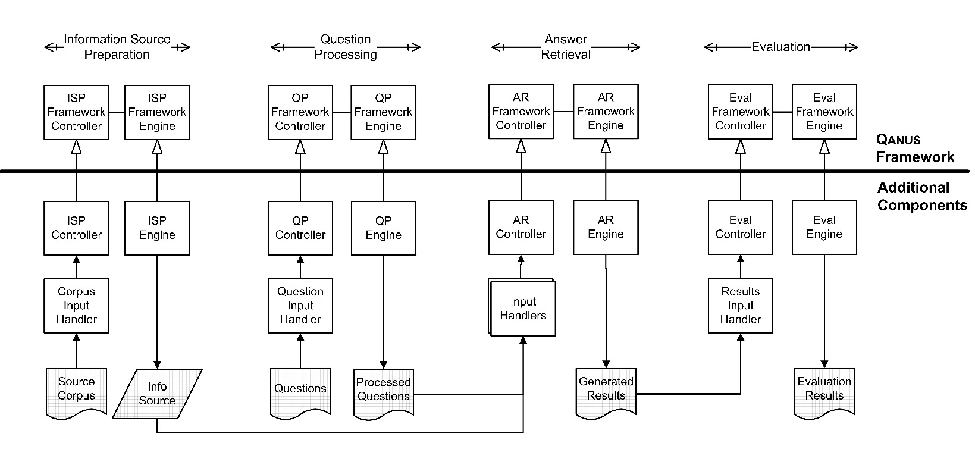
\includegraphics{graficos/Quanus}
  \caption{El framework Quanus y la implementación QA-sys}
  \label{fig:Quanus}
\end{figure}


La arquitectura, al igual que la de DeepQA, es la de un pipeline. Este
sistema consta de tres pasos principales, que se ejecutan todos por
separado (off-line): 


\bigskip

\subsection{Preparación de la fuente de información}
Este paso est\'a pensado para preprocesar cualquier base de conocimiento
y dejarla preparada para el paso 3 (retorno de la pregunta). El
framework se propone tan amplio que no hay m\'as especificaciones al
respecto. La implementaci\'on puntual asume una base de conocimiento en
formato XML de AQUAINT\footnote{\ } y la incorpora a un \'indice de
b\'usquedas Lucene. Este paso incorpora todo el conocimiento que
estar\'a finalmente offline; accesos din\'amicos a la web, por ejemplo,
se modelan en el paso 3.


\bigskip

\subsection{Análisis de la pregunta}
Este paso, igualmente gen\'erico, permite la incorporaci\'on de
distintos componentes para anotar los tokens de la pregunta con datos
\'utiles para ser consumidos por el paso 3. Otro procesamiento a
realizar en este paso podr\'ia ser la generaci\'on de queries
entendibles por los distintos motores de almacenamientos de
informaci\'on del paso 1. En particular, la implementaci\'on trae un
pos-tagger, un ner-tagger y un question classiffier, todos de Stanford.
Hablaremos m\'as de estos componentes m\'as adelante. 


\bigskip

\subsection{Generación de respuestas}
En este paso se utiliza la informaci\'on generada en la preparaci\'on
de la base de informaci\'on y en el procesamiento de la pregunta para
generar una respuesta. Tambi\'en puede incorporarse accesos a la web y
validaciones de las respuestas candidatas. La implementaci\'on concreta
eval\'ua cada pasaje de los primeros n documentos retornados por Lucene
para la pregunta original con una serie de componentes ad-hoc de
distancia para adjudicar diferentes grados de confiabilidad a los
distintos pasajes. \newline


Adem\'as, se provee de un cuarto paso opcional (el sistema de QA est\'a
completo con los tres pasos anteriores), para la fase de desarrollo y
de evaluaci\'on de la performance del sistema:\newline


\subsection{Evaluación}

Este paso est\'a pensado para evaluar las respuestas generadas y
presentarlas de un modo conciso en la fase de desarrollo.
B\'asicamente, cruza las respuestas obtenidas contra unas respuestas
esperadas escritas a mano y presenta el total de respuestas dadas
correctamente.


\bigskip

\subsection{Implementaci\'on}

El c\'odigo est\'a escrito en java y mantiene una interfaz com\'un a
todos los pasos: un controller cuyas responsabilidades son cargar los
componentes y un engine que utiliza los componentes para leer el input,
procesarlo y grabar el resultado. La adaptabilidad del framework est\'a
dada en la posibilidad de incorporar componentes respetando la interfaz
especificada para los mismos o bien, en modificar esta misma interfaz.
Presuntamente, el framework es lo suficientemente abierto para permitir
la implementaci\'on de sistemas basados en distintas fuentes de
conocimiento (ontolog\'ias, archivos, web) y con distintos modos de
funcionamiento mediante poco esfuerzo de customizaci\'on.

La implementaci\'on llamada QA-sys est\'a desarrollada para correr sobre
el tipo de datos de las evaluaciones TREC 2007 (XML AQUAINT). En el
primer paso, incorpora los XML en este formato a un \'indice Lucene, en
el segundo paso utiliza anota la pregunta con POS tags, NERs y
clasifica el tipo de respuesta con un clasificador entrenado y luego,
en el tercer paso se busca la pregunta sobre el \'indice lucene y se
retorna una lista con n documentos rankeados. Estos documentos se
subdividen en pasajes. Luego se aplican diferente algoritmos ad-hoc
dependiendo del tipo de respuesta esperada. \ Por ejemplo, si la
respuesta es un nombre de persona, se ejecuta NER sobre los diferentes
pasajes buscando nombres candidatos, si el tipo esperado es una fecha,
se utilizan expresiones regulares escritas a mano, etc. Finalmente, los
pasajes candidatos se eval\'uan utilizando heur\'isticas de proximidad
de los candidatos a la pregunta inicial. Para esto se utilizan
diferentes Scorers que rankean los pasajes seg\'un diferentes
caracter\'isticas (features) y luego se selecciona alguna priorizando
algunas caracter\'isticas sobre otras, dependiendo tambi\'en del tipo
de respuesta esperada. Por \'ultimo, el evaluador de resultados mide la
exactitud (\textit{accuracy}): total de respuestas correctas sobre
total de preguntas. QA-sys funciona s\'olo sobre preguntas del tipo
factoid y, a modo de comparaci\'on, el mejor sistema seg\'un la TREC
2007, el LymbaPA07 obtuvo un grado de exactitud del 0.706 y el d\'ecimo
(Quanta) obtuvo 0.206, mientras que QA-sys logra el 0.119. La
implementaci\'on es realmente simple y funciona s\'olo a modo de
ilustraci\'on de lo que puede construirse sobre el framework. 

\bigskip

\section{Otros sistemas de QA: OpenEphyra, Aranea y Just.Ask}

\bigskip

El paper describe las arquitecturas de todos los sistemas, si sirve
meter m\'as info

El paper [EPHYRA1] \ busca crear un criterio cuantitativo para comparar
la eficacia de distintos pasos de Just.Ask, Open Ephyra y Aranea
bas\'andose en la arquitectura \textit{pipeline de tres pasos}
compartida por todos. Los tres sistemas, por lo dem\'as, est\'an
basados en la web, utilizando distintas APIs de buscadores o bien
analizando los resultados de la interfaz de usuario de los mismos. 

El primer \'item importante a destacar de este trabajo, es que, al
momento de la experimentaci\'on \textbf{Aranea no funcionaba m\'as y
estaba discontinuado}\footnote{\ (Resaltado en Secci\'on 8, muy
concluyente).\par }\textbf{. }El autor se comunic\'o con el responsable
del proyecto que corrobor\'o que las APIs de los buscadores en los que
se basaba Aranea cambiaron y no hab\'ia inter\'es en readaptar el
c\'odigo para que vuelva a funcionar. Las comparaciones que logr\'o
entre Just.Ask y Open Ephyra son interesantes y concluyentes a favor de
la performance de OpenEphyra. 

(Freeling \ + Cambio de Base + Rigidez)
